\providecommand{\main}{..}
\documentclass[\main/Tesi.tex]{subfiles}
\begin{document}
\chapter{Strumenti}

La scelta degli strumenti è stata fortemente condizionata da codebase preesistenti.\\
I programmi nei quali la soluzione sarà integrata sono scritti in C\# utilizzando il framework per lo sviluppo di interfacce grafiche \textbf{Windows Presentation Foundation} \cite{wpf} e in particolare si basano sul .NET Framework, l'implementazione originale del runtime .NET disponibile solo per Windows.\\
Questa condizione di partenza ha creato alcuni limiti di sviluppo (ad esempio di compatibilità con nuove librerie o tool di sviluppo) e resi necessari alcuni cambiamenti (vedi \ref{refactor}) nei progetti preesistenti per poter sviluppare dei componenti moderni e che siano adeguati alla transizione tra .NET Framework e il più recente .NET Core.

\section{Ecosistema e linguaggi}
\subsection{.NET}
.NET è un ecosistema di sviluppo software creato da Microsoft negli anni 2000 come alternativa a Java. Si basa su un runtime che esegue un bytecode intermedio chiamato \textbf{CIL} \cite{cil} attraverso una macchina virtuale o un compilatore Just in Time.\\
Questo tipo di implementazione consente il supporto a multipli linguaggi di programmazione interoperabili tra di loro (con l'unico vincolo di essere compilabili in CIL) che possono essere eseguiti su qualsiasi sistema operativo per il quale esista una versione del runtime.

\begin{figure}[h]
\caption{Funzionamento del .NET runtime, dal web.}
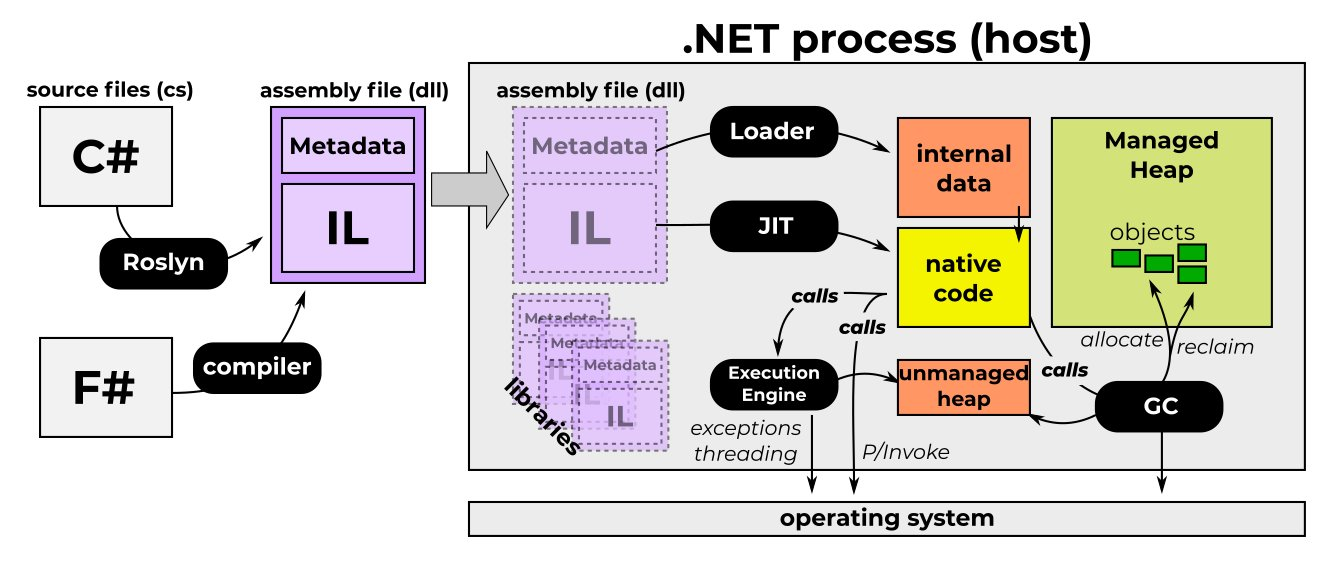
\includegraphics[width=\textwidth]{../images/dotnet.png}
\end{figure}

Fino al 2015, ufficialmente questo ecosistema era utilizzabile solo su Windows (sotto il nome di .NET Framework), ma in seguito Microsoft sviluppò e rese open source una nuova versione, chiamata .NET Core, più veloce e moderna ma soprattutto multipiattaforma.
I software nei quali la soluzione sviluppata è stata in seguito integrata utilizzavano la versione 4.5.2 del .NET Framework, una versione discretamente vecchia.\\
Data la volontà di sviluppare il modulo in chiave moderna, è stata presa la decisione di consolidare (vedi \ref{refactor} e \ref{nuget}) questi software per integrarlo nel modo più semplice possibile, visto il pesante utilizzo che se ne sarebbe fatto.\\
Si è quindi deciso di sviluppare il modulo in .NET Standard, un set di API comune tra tutte le implementazioni di .NET (CLR, CoreCLR e Mono) che assicura la portabilità del codice tra diversi runtime e sistemi operativi.\\
Una libreria .NET Standard 2.0 necessita, per essere consumata dal .NET Framework, almeno della versione 4.6.1, rendendo necessario l'upgrade degli altri progetti ad una versione superiore, in questo caso è stata scelta la 4.7.2.\\
Inoltre, tutte le librerie preesistenti non legate a Windows (quindi principalmente dominio, gestione della persistenza e servizi) sono state convertite a .NET Standard.\\
Questi passaggi sono essenziali per un futuro upgrade dei progetti a .NET Core, la nuova versione di .NET multipiattaforma.\\
Per di più hanno consentito un upgrade del formato dei file di configurazione dei progetti (il passaggio da .NET Framework a .NET Standard/Core ha aggiornato la sintassi e le funzionalità dei file \textit{.csproj}, ossia i file che identificano un progetto .NET, rendendoli più compatti ed eliminando la necessità di utilizzare file di configurazione ulteriori) e permesso di utilizzare le ultime versioni del linguaggio scelto, ossia C\#.

\subsection{C\#}
C\# è il linguaggio .NET più famoso ed utilizzato. Nato come linguaggio puramente ad oggetti, si è in seguito allontanato da Java preferendo un approccio multi-paradigma e, nelle ultime versioni, sempre più funzionale.
La versione di C\# utilizzata per il modulo è la 9, l'ultima disponibile durante lo sviluppo ed è in opposizione alla versione utilizzata nei progetti target del modulo, ossia la 7.3.\\
La differenza tra le due è molto marcata, in quanto le più recenti versioni introducono due feature largamente utilizzate durante lo sviluppo del modulo:
\begin{itemize}
    \item \textbf{Recursive Patterns} \cite{recursivepatterns}: una feature ispirata alla keyword \textbf{match} dei linguaggi funzionali, consente di fare confronti ricorsivi ed esauistivi sulle proprietà degli oggetti.\\Consente di effettuare controlli complessi e su diversi livelli di profondità con una sintassi molto corta, concisa e ispirata alla sintassi della lingua inglese.\\Sono inoltre espressioni contestuali, si possono infatti concatenare multipli controlli di diverso tipo alla stessa variabile o gruppo di variabili.\\Questa feature è stata fortemente utilizzata durante la serializzazione e deserializzazione da database.
    \item \textbf{Nullable Reference Types} \cite{nullable}: Si tratta di annotazioni sulle dichiarazioni dei tipi degli oggetti, che identificano se un oggetto può o meno essere nullo.\\Queste annotazioni portano lo sviluppatore a prestare una maggiore attenzione al design del software, costringendolo ad assicurarsi che deterministicamente ogni singolo oggetto abbia un riferimento di memoria valido o che, nel caso non sia così, sia una situazione gestita.\\È stata una feature essenziale durante lo sviluppo in quanto ha ridotto al minimo le referenze errate.
\end{itemize}

\section{Framework e Librerie}

\subsection{Windows Presentation Foundation}
WPF è il framework per la progettazione di applicazioni con interfaccia grafica più utilizzato nel mondo .NET.\\
Si basa sull'utilizzo del linguaggio di markdown \textbf{XAML} \cite{xaml} (in coppia con C\#) per la definizione dell'interfaccia e del pattern MVVM (Model - View - ViewModel) \cite{mvvm} per l'aggiornamento della UI al cambiare dei dati.\\
La conoscenza di questo framework è risultata essenziale nella fase avanzata dello sviluppo, durante la quale il componente, fino ad allora sviluppato esternamente, è stato integrato nei software esistenti e di conseguenza con WPF.

\subsection{Entity Framework Core}
\label{efcore}
La libreria più impattante nello sviluppo della soluzione è stata \textbf{Entity Framework Core} (abbreviato EFCore) \cite{efcore}, l'\textbf{ORM} (Object Relational Mapping) di Microsoft e una garanzia del mondo .NET, che fornisce tutti gli strumenti necessari per la comunicazione con i database.\\
Un ORM è un infatti livello di astrazione tra database relazionali e linguaggi ad oggetti che permette di utilizzare solo codice del linguaggio target (in questo caso C\#) invece del classico SQL. I vantaggi sono molti, tra i quali troviamo:
\begin{itemize}
    \item Una maggiore manutenibilità e correttezza, in quanto normalmente il codice SQL viene salvato in semplici stringhe senza alcun sistema di linting o segnalazione di errori in fase di compilazione, mentre nel caso degli ORM è puro codice del linguaggio target supportato quindi da tutti i tool di sviluppo.
    \item Una maggiore semplicità e consistenza dei tipi.
    \item Una serie di automatismi, come la creazione del database e della sua struttura (tabelle e viste).
    \item Supporto a multipli DBMS con pochi o nessun cambiamento a livello di codice.
    \item Maggiore sicurezza, in quanto ogni query è compilata e il suo contenuto controllato per evitare codice malevolo o sintatticamente errato.
\end{itemize}

\begin{figure}[h]
\caption{Esempio di mappatura tra entità e classi effettuato da un ORM}
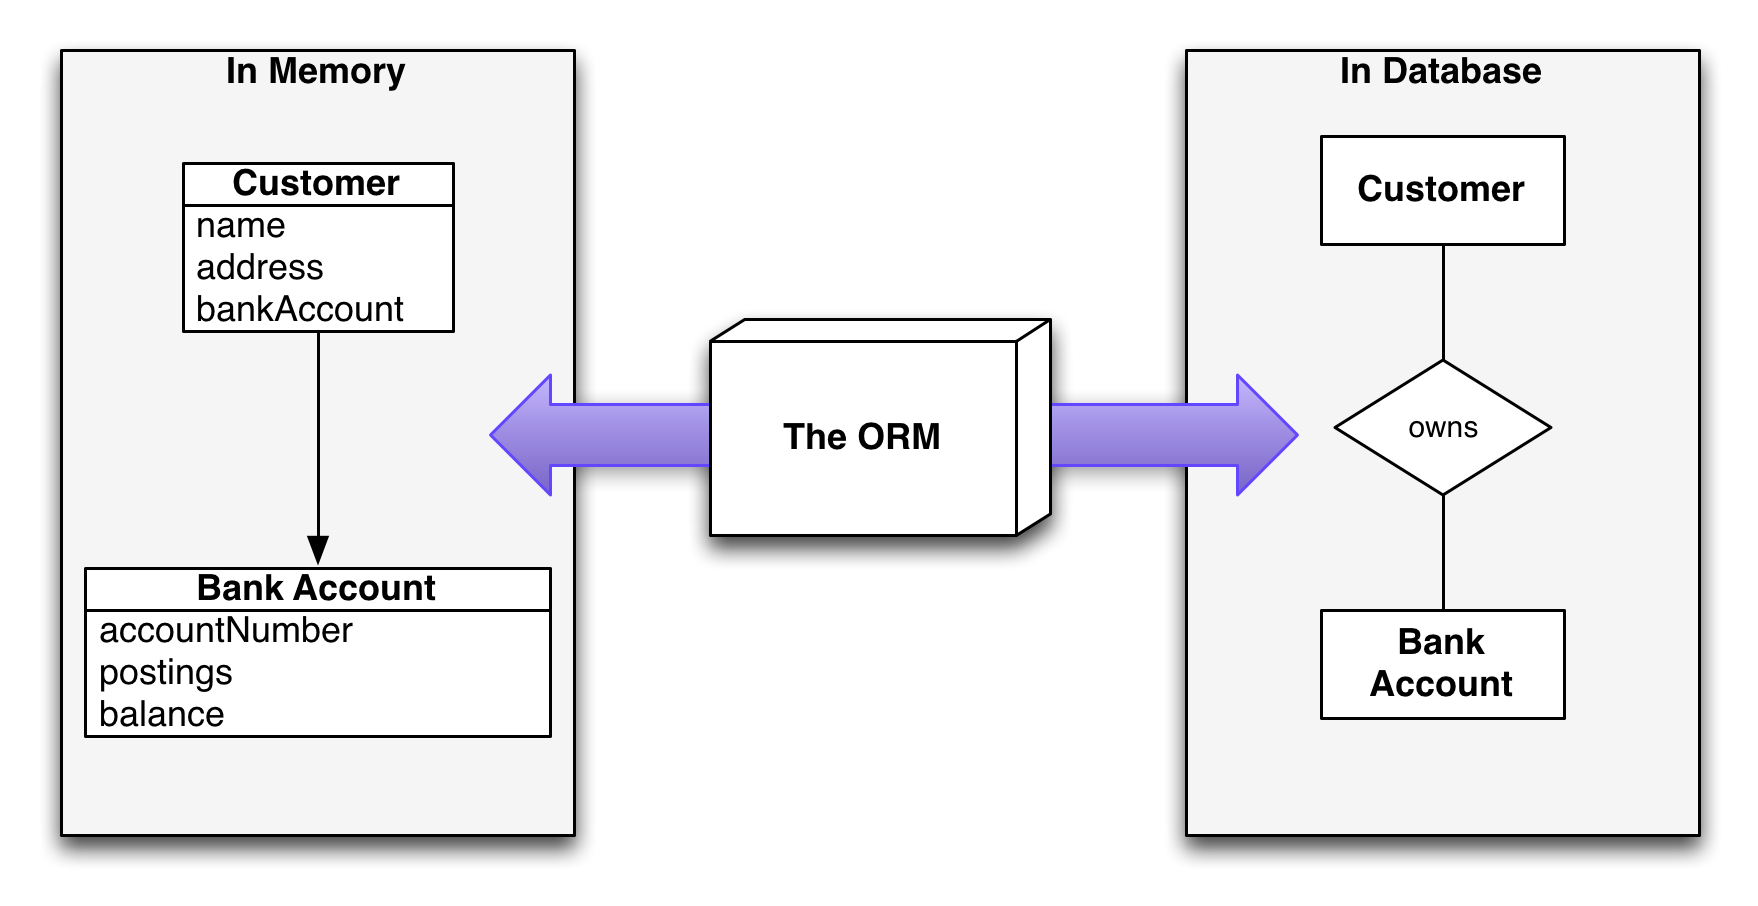
\includegraphics[width=\textwidth]{../images/orm.png}
\end{figure}

In particolare Entity Framework è famoso per la sua integrazione con \textbf{Linq} \cite{linq}, un linguaggio di query simile ad SQL ma completamente integrato in C\# e che fornisce anche un set di metodi alternativi completamente \textit{funzionali}.\\
Questo, unito al sistema di tipi statici di C\#, garantisce una semplice e solida alternativa all'utilizzo di normali query SQL.\\
Ovviamente, l'utilizzo di un sistema del genere prevede una perdita di performance ma, a differenza della maggior parte degli ORM, EFCore utilizza alcuni strumenti di metaprogramming forniti dall'ecosistema per ridurre al minimo l'overhead e limitarlo solo alla prima esecuzione, durante la quale le query Linq vengono analizzate e trasformate in effettive stringhe SQL.\\
Versioni successive di EFCore rispetto a quella utilizzata effettuano questa fase a compile time.\\
EFCore supporta svariati providers, ossia astrazioni che permettono a diversi DBMS di supportare pienamente il framework.\\
Questa funzionalità è stata ampliamente utilizzata per condividere la maggioranza del codice di interfacciamento con il database centrale e quello locale.\\
Difatti lo stesso \textbf{DbContext}, ossia la classe che rappresenta l'intero database, può essere riutilizzato con diversi DBMS o diverse istanze dello stesso modificando semplicemente la stringa di connessione e di conseguenza, creando istanze con parametri diversi è stato possibile supportare entrambi i database.\\
Sono state valutate possibili alternative, tra le quali la versione precedente denominata semplicemente "Entity Framework". Nonostante sia una versione più rodata e completa a livello di funzionalità, è molto meno flessibile ed è al momento supportata solo a livello di manutenzione e in futuro sarà probabilmente deprecata.\\
La versione utilizzata di Entity Framework Core è la `3.1`, l'ultima supportata da .NET Framework. È una versione LTS, quindi il suo supporto sarà esteso e legato al supporto della corrispondente versione di .NET Core, ossia fine 2022, un tempo sufficiente per migrare tutti i software e le librerie al nuovo .NET 6, ossia la versione LTS successiva.\\
Altre funzionalità chiave del framework utilizzate ampliamente sono:
\begin{itemize}
    \item Le \textbf{transazioni}, supportate allo stesso modo dei principali DBMS, consentono di eseguire scritture a database avendo la possibilità di tornare ad uno stato precedente in caso di errore.
    \item Le \textbf{migrazioni}, che consistono nell'applicare modifiche alla struttura del database con il cambiare delle versioni del programma senza perdere i dati contenuti in database di versioni preesistenti.\\
    Una migrazione consiste nel generare codice target (quindi in questo caso, C\#) che esegue operazioni di update delle tabelle, codice che viene aggiornato ad ogni cambiamento della struttura del database durante lo sviluppo.\\
    Nonostante la struttura del database sia molto semplice e difficilmente sarà soggetta a modifiche, averne la possibilità a costo zero è un plus.
\end{itemize}

\subsection{Newtonsoft.Json}
La libreria di manipolazione delle stringhe in formato \textbf{JSON} \cite{json} più utilizzata dagli sviluppatori .NET, consente in una riga di codice di serializzare da oggetto a JSON o deserializzare da json ad oggetto con ottime prestazioni.\\
Consente inoltre di creare facilmente serializzatori e deserializzatori custom per poter gestire casi speciali.

\subsection{Logging}
Il logging è parte essenziale di un software moderno, che necessita di tracciabilità degli errori ed eventi.\\ 
L'azienda ne faceva già uso estensivo ed organizzato negli altri software, dividendo i log sia per tipo che per importanza.\\
Nel mondo .NET il logging è gestito utilizzando due moduli separati.\\
\begin{itemize}
    \item Il primo è composto da una serie di astrazioni, ossia interfacce che rappresentano una standardizzazione delle funzionalità di logging (ad esempio la scelta della priorità dell'output).\\I software preesistenti utilizzano le astrazioni fornite dalla libreria open source \textbf{Common.Logging}, ormai non più mantenuta.\\In previsione di una migrazione totale la soluzione è stata sviluppata utilizzando la libreria di Microsoft, ossia \textbf{Microsoft.Extensions.Logging}, che permette un'integrazione con EFCore e i tools di Inversion of Control che saranno illustrati in nella sezione \ref{ioc}.
    \item Il secondo è il cosiddetto provider, ossia l'effettiva implementazione delle astrazioni, che solitamente richiede un file di configurazione.\\In questo caso è stato mantenuto il provider utilizzato nei software nei quali è stata integrata la soluzione, ossia la libreria \textbf{NLog}, che supporta entrambe le astrazioni citate in precedenza.
\end{itemize}

\section{Database}

\subsection{SQL Server}
A livello di database centrale l'azienda utilizza da sempre \textbf{SQL Server} \cite{mssql} per le sue applicazioni, solitamente per i dati relativi ai pazienti, ed è stato quindi deciso di utilizzare questo DBMS anche in questo caso per la gestione centrale dei settaggi.\\
SQL Server garantisce il supporto a \textbf{multiple istanze, concorrenza, alte performance e bassa latenza} nelle richieste.\\
Fornisce inoltre svariati strumenti di sviluppo e debugging, tra i quali il supporto completo ad EFCore.\\

\subsection{SQLite}
Per quanto riguarda il database locale al singolo programma, è stato scelto \textbf{SQLite} \cite{sqlite}, un DBMS molto più semplice e limitato di SQL Server e simili, ma che \textbf{non richiede un'installazione globale}, essendo tutto il codice necessario al funzionamento contenuto nel driver distribuito assieme all'applicazione.\\
Garantisce comunque ottime performance e fornisce una libreria per il supporto ad EFCore.

\section{Pattern e Principi software}

\subsection{Inversion of Control e Dependency Injection}
\label{ioc}
L'\textbf{Inversion of Control} \cite{ioc} è un principio di programmazione che consiste nell'ottenimento del controllo dei componenti riutilizzabili da parte di componenti specifici dell'applicazione, contrariamente a quanto accade solitamente dove è il componente di livello più alto a lasciare il controllo ad uno dedicato.\\
Questo principio è largamente utilizzato nei linguaggi ad oggetti e in particolare nei framework dedicati allo sviluppo di sistemi web lato server dove viene implementato attraverso le cosiddette \textbf{Dependency Injection}, sistema che consente di \textit{iniettare} le istanze dei \textit{servizi} direttamente come parametri dei costruttori o proprietà degli oggetti.\\

\begin{figure}[h]
\caption{Il funzionamento delle Dependency Injection}
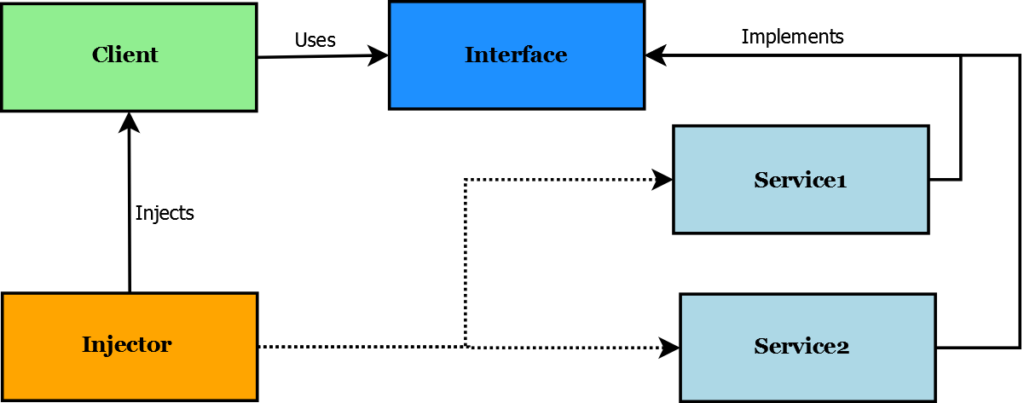
\includegraphics[width=\textwidth]{../images/ioc.png}
\end{figure}

Per quanto concerne questo progetto, è stata utilizzata la libreria ufficiale fornita da Microsoft, \textbf{Microsoft.Extensions.DependencyInjection}, da scaricare separatamente ma considerata parte del runtime (si trova infatti nello stesso repository open source del runtime .NET) e che consente le "iniezioni" a livello di costruttore.\\
Questa libreria permette di registrare servizi (che saranno in seguito iniettati) di 3 livelli diversi:
\begin{itemize}
    \item \textbf{Singleton}: Oggetti che possiedono un \textit{lifetime} pari a quello del programma e di cui esiste una singola istanza.
    \item \textbf{Transient}: Oggetti dei quali viene creata un'istanza per ogni richiesta che però persiste finchè non disposta manualmente.
    \item \textbf{Scoped}: Oggetto il cui \textit{lifetime} dura lo stretto necessario per compiere una \textbf{Unit of Work} \cite{uow}.
\end{itemize}
Queste differenze sono essenziali in un progetto del genere dove ogni componente ha un \textit{lifetime} preciso per garantire ottimizzazione e ed evitare accumuli di memoria in caso di sessioni durature.\\
È inoltre un sistema molto comodo per facilitare il \textbf{loose coupling}, principio del software che consiste in componenti che conoscono il minimo indispensabile l'uno dell'altro, trascurando i dettagli implementativi e riducendo al minimo funzioni e proprietà esposte.\\
È lo standard per applicazioni .NET a livello industriale come il progetto in questione. 

\subsection{Model View ViewModel}
\label{mvvm}
Il pattern \textbf{MVVM} consiste nell'associare ogni componente dell'applicazione ad una di tre categorie, le quali interagiscono tra di loro secondo uno schema ben preciso:
\begin{itemize}
    \item \textbf{Model}: Il dominio dell'applicazione, ossia modelli passivi i quali hanno lo scopo di contenere e rappresentare dati. Non contengono alcun tipo di logica funzionale.
    \item \textbf{View}: La definizione dell'interfaccia grafica dell'applicazione, nel caso di WPF si tratta di codice XAML. Esattamente come i modelli, non contiene logica funzionale.
    \item \textbf{ViewModel}: Il collante tra View e Model, si può definire come il controllore di uno specifico caso d'uso e colui che si occupa di collegare (attraverso i cosiddetti \textit{Binding}) istanze dei modelli a componenti della view.
\end{itemize}
WPF supporta nativamente il pattern MVVM.\\
Infatti, lo XAML supporta il concetto di Binding tra una proprietà di un componente della UI (ad esempio un bottone) in modo che i valori del modello siano rispecchiati nella struttura della UI.\\
È essenziale però che cambiamenti nei dati siano rispecchiati nella UI e a volte viceversa (come nel caso di un modello collegato ad un input di testo) ed in questo il pattern MVVM aiuta grazie alla separazione degli stati, che permette di non confondere le logiche funzionali (che avvengono solo nel ViewModel) con le logiche di sviluppo della UI, che sono (nel caso di WPF) gestite dallo XAML.\\

\begin{figure}[h]
\caption{La struttura Model View ViewModel}
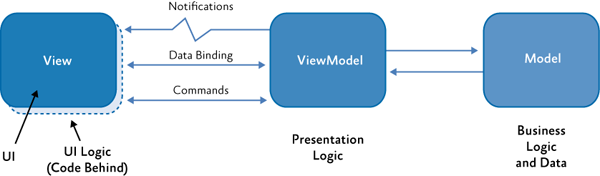
\includegraphics[width=\textwidth]{../images/mvvm.png}
\end{figure}

In particolare, per gestire cambiamenti di singoli oggetti si utilizza l'interfaccia \textbf{INotifyPropertyChanged}, che specificherà alla View quale variabile si è aggiornata in modo che possa ricaricare gli elementi con i quali è stato effettuato il binding con i valori più aggiornati.\\
Diversamente, per gestire modifiche a collezioni (alle quali vengono aggiunti o tolti elementi) si utilizza l'\textbf{ObservableCollection}, una lista che implementa l'interfaccia appena specificata.\\
Inoltre, nel caso di manipolazioni della UI non esprimibili in XAML e che non riguardano alcun tipo di controllo di flusso funzionale (come ad esempio la creazione di certi effetti estetico), WPF aggiunge il concetto di Controller, una classe che estende la View. \\
Per garantire un'integrazione del nuovo modulo all'interno dei programmi esistenti, supportare il pattern MVVM, in particolare le implementazioni .NET, è essenziale.

\section{Strumenti di sviluppo}

\subsection{IDE e Text Editors}
Nell'ecosistema .NET, \textbf{Visual Studio} è l'IDE standard utilizzato ed è infatti stato mantenuto come software di riferimento per lo sviluppo.\\
La versione minima necessaria è la 2019 (l'unica che supporta versioni di C\# recenti).\\
Essendo però .NET Standard legato a .NET Core, Visual Studio non è un requisito necessario, infatti anche altri IDE e Text Editor lo supportano, in particolare è stata testata la piena compatibilità con \textbf{Visual Studio Code} \cite{vscode}, uno dei text editor più famosi ed utilizzati.\\
Degno di menzione è \textbf{SQL Server Management Studio} \cite{visualstudio}, che è stato utilizzato per il testing dell'integrità dei dati durante lo sviluppo.

\subsection{Nuget Package Manager}
\textbf{Nuget} \cite{nuget} è il nome del più popolare package manager utilizzato nel mondo .NET.\\
Non solo è stato utilizzato per la gestione dei pacchetti pubblici forniti da Microsoft o terze parti (contenuti nel repository principale residente in nuget.org), ma anche per il riutilizzo di codice interno all'azienda tra i diversi progetti.\\
Nuget consente infatti la creazione di pacchetti da salvare in un server locale o HTTP, per essere consumati da qualsiasi progetto, semplificando la condivisione di librerie.\\

\subsection{Versioning e Task Management}
Nello sviluppo software, gli strumenti di versioning sono vitali per la gestione di progetti complessi.\\
Permettono infatti di sincronizzare il lavoro di multipli sviluppatori sullo stesso codice.\\
Ma è anche necessario tenere traccia di bug, feature e versioni.\\
Il sistema \textbf{IBM Rational} \cite{rational} soddisfa tutti questi requisiti permettendo un hosting locale (necessario in ambito bio-medicale) e strumenti aggiuntivi per la gestione di progetti hardware e documentazione.\\
Fornisce inoltre una base per la Continuous Integration/Continuous Deployment. 

\subsection{Testing e Test Lab}
Come spiegato nella sezione \ref{testing}, l'azienda deve sottostare a degli standard qualitativi molto alti nello sviluppo software, di conseguenza il testing è una parte essenziale dei suoi prodotti.\\
Possiede perciò un \textbf{Test Lab} molto articolato e composto soprattutto di testing manuale, avendo a che fare con macchinari difficilmente simulabili.\\
Per quanto riguarda invece il territorio dei test automatici, è stato utilizzato il framework \textbf{xUnit} \cite{xunit}, in particolare per \textit{Unit Test} e \textit{Integration Test}.\\
Come possibili alternative sono stati valutati anche \textbf{MSTest} (Ufficiale di Microsoft) e \textbf{NUnit}, ma il framework scelto si è rivelato più estensibile e semplice da utilizzare.

\subsection{CI/CD}
Come accennato in precedenza, Continuous Integration e Deployment sono gestiti da IBM Rational, che fornisce una serie di software supplementari che consentono di eseguire task di build e deployment dei software sviluppati, sia manualmente che in automatico, utlizzando specifici trigger (come ad esempio il "delivery" di una nuova versione del codice).\\
Sono presenti due macchine virtuali con ruoli dedicati:
\begin{itemize}
    \item Una è dedicata al build, scarica gli ultimi cambiamenti a livello di codice ed esegue uno script contenuto nel codice sorgente.\\Il risultato della compilazione viene poi caricato automaticamente in una sezione di Rational dedicata ai file binari.
    \item L'altra macchina virtuale si occupa invece del deploy automatico, utilizza i file creati dalla precedente compilazione e li utilizza per creare un pacchetto di installazione utilizzando il software \textbf{InstallShield} \cite{installshield}.
\end{itemize}

\begin{figure}[h]
    \caption{Un'immagine descrittiva del flusso di esecuzione della Continuous Integration/Continuous Delivery di Micromed.}
    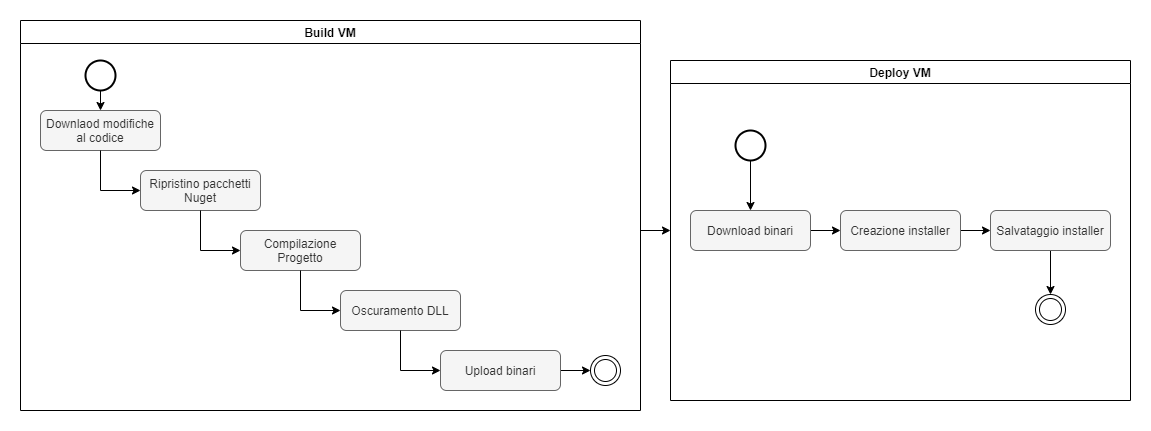
\includegraphics[width=\textwidth]{../images/ci.png}
\end{figure}

Il pacchetto risultante viene poi salvato in una sezione apposita di IBM Rational che mantiene lo storico di tutte le versioni rilasciate.

\end{document}